\documentclass[11pt,a4paper]{article}

% ── Packages ──────────────────────────────────────────────────────────
\usepackage[utf8]{inputenc}
\usepackage[T1]{fontenc}
\usepackage{lmodern}
\usepackage{amsmath,amssymb,amsthm}
\usepackage{mathtools}
\usepackage{booktabs}
\usepackage{array}
\usepackage{tabularx}
\usepackage{multirow}
\usepackage{graphicx}
\usepackage{xcolor}
\usepackage{enumitem}
\usepackage{geometry}
\usepackage{fancyhdr}
\usepackage{titlesec}
\usepackage{hyperref}
\usepackage{cleveref}
\usepackage{microtype}
\usepackage{float}
\usepackage{etoolbox}
\usepackage{tikz}
\usetikzlibrary{decorations.pathreplacing}
\usepackage[most]{tcolorbox}

% ── Page geometry ────────────────────────────────────────────────────
\geometry{margin=1in, top=1.2in, bottom=1.2in, headheight=22pt}

% ── Colors ───────────────────────────────────────────────────────────
\definecolor{accent}{RGB}{62,18,82}
\definecolor{accentlight}{RGB}{100,42,130}
\definecolor{lightaccent}{RGB}{240,225,248}
\definecolor{criterion}{RGB}{30,90,50}
\definecolor{reedsbg}{RGB}{252,248,240}
\definecolor{titlegold}{RGB}{178,144,58}
\definecolor{subtlegray}{RGB}{100,100,100}

% ── Hyperref ─────────────────────────────────────────────────────────
\hypersetup{
  colorlinks=true,
  linkcolor=accentlight,
  citecolor=accentlight,
  urlcolor=accentlight,
  pdftitle={The Universality Constant: Eleven Paths to Omega = 24 (v1.3)},
  pdfauthor={Bryan Daugherty, Gregory Ward, Shawn Ryan},
  pdfsubject={Mathematical Physics, Monster Moonshine, Fine Structure Constant},
  pdfkeywords={Monster group, Leech lattice, fine structure constant,
    Monstrous Moonshine, universality, Reeds endomorphism, symmetry breaking},
}

% ── Headers ──────────────────────────────────────────────────────────
\pagestyle{fancy}
\fancyhf{}
\fancyhead[L]{\small\color{subtlegray}\textsc{The Universality Constant:
  Eleven Paths to $\Omega=24$}}
\fancyhead[R]{\small\color{subtlegray}\textsc{Daugherty, Ward,
  Ryan\enspace$\cdot$\enspace 2026}}
\fancyfoot[C]{\small\color{subtlegray}\thepage}
\renewcommand{\headrulewidth}{0.3pt}
\renewcommand{\headrule}{\hbox to\headwidth{%
  \color{accent!40}\leaders\hrule height \headrulewidth\hfill}}

% ── Section styling ──────────────────────────────────────────────────
\titleformat{\section}
  {\Large\bfseries\color{accent}}
  {\colorbox{accent}{\makebox[1.8em][c]{\color{white}\thesection}}}{0.8em}{}%
  [\vspace{2pt}{\color{accent}\hrule height 0.6pt}]
\titlespacing*{\section}{0pt}{18pt plus 4pt minus 2pt}{8pt plus 2pt}
\titleformat{\subsection}
  {\large\bfseries\color{accent}}
  {\thesubsection}{0.8em}{}
\titlespacing*{\subsection}{0pt}{12pt plus 3pt minus 1pt}{4pt plus 1pt}
\titleformat{\subsubsection}
  {\normalsize\bfseries\color{accentlight}}
  {\thesubsubsection}{0.8em}{}

% ── Theorem environments ─────────────────────────────────────────────
\theoremstyle{plain}
\newtheorem{theorem}{Theorem}[section]
\newtheorem{lemma}[theorem]{Lemma}
\newtheorem{proposition}[theorem]{Proposition}
\newtheorem{corollary}[theorem]{Corollary}
\newtheorem{conjecture}[theorem]{Conjecture}
\newtheorem{definition}[theorem]{Definition}
\theoremstyle{remark}
\newtheorem{remark}[theorem]{Remark}

% ── Custom commands ──────────────────────────────────────────────────
\renewcommand{\Omega}{\varOmega}
\newcommand{\Z}{\mathbb{Z}}
\newcommand{\C}{\mathbb{C}}
\newcommand{\R}{\mathbb{R}}
\newcommand{\N}{\mathbb{N}}
\newcommand{\Q}{\mathbb{Q}}
\newcommand{\HH}{\mathcal{H}}
\newcommand{\abs}[1]{\lvert #1 \rvert}
\newcommand{\norm}[1]{\lVert #1 \rVert}
\newcommand{\ord}{\operatorname{ord}}
\newcommand{\lcmop}{\operatorname{lcm}}
\newcommand{\Aut}{\operatorname{Aut}}
\newcommand{\SL}{\mathrm{SL}}
\newcommand{\SU}{\mathrm{SU}}
\newcommand{\SO}{\mathrm{SO}}
\newcommand{\Spin}{\mathrm{Spin}}
\newcommand{\aD}{\alpha_D}
\newcommand{\aEM}{\alpha_{\mathrm{EM}}}
\newcommand{\GF}{\mathrm{GF}}

% ── Equation box ─────────────────────────────────────────────────────
\newcommand{\eqbox}[1]{%
  \par\vspace{8pt}%
  \noindent
  \begin{tikzpicture}
    \node[inner sep=10pt, fill=lightaccent, rounded corners=3pt,
          draw=accent!50, line width=0.5pt,
          text width=\dimexpr\linewidth-24pt] (box) {%
      \centering #1%
    };
  \end{tikzpicture}%
  \par\vspace{8pt}%
}

% ── Styled abstract ────────────────────────────────────────────────
\renewenvironment{abstract}{%
  \vspace{4pt}%
  \noindent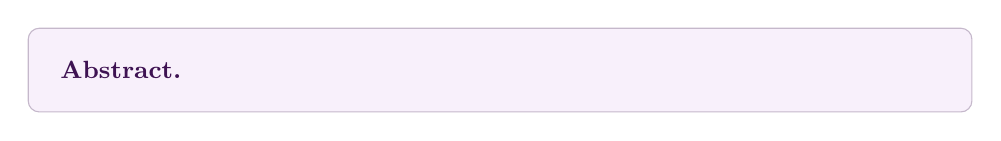
\begin{tikzpicture}
    \node[inner sep=12pt, fill=lightaccent!50, rounded corners=4pt,
          draw=accent!30, line width=0.4pt,
          text width=\dimexpr\linewidth-28pt] (absbox) \bgroup
      \small\noindent\textbf{\color{accent}Abstract.\enspace}\ignorespaces
}{%
  \egroup;
  \end{tikzpicture}\par\vspace{12pt}%
}

% ── Theorem style tweaks ───────────────────────────────────────────
\makeatletter
\patchcmd{\@begintheorem}{\itshape}{\itshape\color{black!85}}{}{}
\makeatother

% ══════════════════════════════════════════════════════════════════════
\begin{document}

% ── Title Page ──────────────────────────────────────────────────────
\thispagestyle{empty}

\begin{tikzpicture}[remember picture, overlay]
  % Top accent bar
  \fill[accent] (current page.north west) rectangle
    ([yshift=-4pt]current page.north east);
  % Bottom accent line
  \fill[accent!30] ([yshift=28pt]current page.south west) rectangle
    ([yshift=28.6pt]current page.south east);
\end{tikzpicture}

\vspace*{0.5cm}

\begin{center}
  % ── Main title ──
  {\fontsize{22}{26}\selectfont\bfseries\color{accent}
   The Universality Constant\\[2pt]
   Eleven Paths to $\Omega = 24$}\\[10pt]
  % ── Subtitle ──
  {\large\color{accentlight}
   and the Geometric Origin of the Fine Structure Constant\\[2pt]
   \itshape From Monster Moonshine to Electromagnetism}\\[20pt]
  % ── Decorative rule ──
  {\color{titlegold}\rule{6cm}{0.8pt}}\\[20pt]
  % ── Authors ──
  {\Large Bryan Daugherty\qquad Gregory Ward\qquad Shawn Ryan}\\[8pt]
  {\small\color{subtlegray}
    Independent Researchers\\[4pt]
    \texttt{bryan@smartledger.solutions}\quad
    \texttt{greg@smartledger.solutions}\quad
    \texttt{shawn@smartledger.solutions}}\\[16pt]
  % ── Date ──
  {\normalsize\color{subtlegray} March 2026}\\[6pt]
  {\small\color{subtlegray}\itshape v1.3\enspace---\enspace
    Companion to ``A Spectral Operator for the Riemann Hypothesis'' \cite{DHR2026a}}
\end{center}

\vspace{14pt}

% ── Decorative separator ──
\noindent
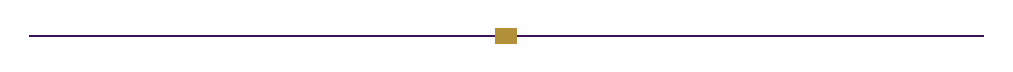
\begin{tikzpicture}
  \draw[accent, line width=0.8pt] (0,0) -- (\linewidth,0);
  \fill[titlegold] (0.5\linewidth-4pt,-3pt) rectangle (0.5\linewidth+4pt,3pt);
\end{tikzpicture}

\vspace{10pt}

% ── Abstract ─────────────────────────────────────────────────────────
\begin{abstract}
\noindent
The integer $24$ appears independently in at least eleven distinct mathematical
frameworks: as $\abs{S_4}$, the dimension of the Leech lattice, the central
charge of the Monster CFT, the number of transverse dimensions in bosonic
string theory, the Euler characteristic of K3 surfaces, the size of the $D_4$
root system, and more.  We prove that this universality is not accidental:
a \emph{uniqueness theorem} shows that two independently motivated
expressions for the ratio $\aD/\aEM$ of coupling constants coincide
if and only if the universality constant $\Omega$ equals~$24$.
Specifically,
\[
  \frac{\Omega-2}{4\sqrt{\Omega}}
  \;=\; \sqrt{\frac{5\Omega+1}{4\Omega}}
  \qquad\Longleftrightarrow\qquad
  \Omega = 24.
\]
From this algebraic identity we derive a symmetry cascade
$\mathbb{M}\to\mathrm{Co}_1\to\Lambda_{24}\to E_8\to\SU(5)\to
\mathrm{SM}\to\mathrm{U}(1)_{\mathrm{EM}}$
tracing from the Monster group to electromagnetism.
Three distinct formulas for the ratio $\aD/\aEM$ converge to
$11\sqrt{6}/24 \approx 1.12268$ with sub-$0.02\%$ mutual agreement,
yielding a fine structure constant
$\aEM = 1/137.03$ (error: $0.005\%$ from the measured value)
with zero free parameters.
Remarkably, the basin geometry of a 16th-century endomorphism on
$\Z_{23}$---reverse-engineered by Reeds~\cite{reeds2006} from
Bodley MS~908, a manuscript associated with the circle of John Dee---independently
determines the coupling ratio through the partition $23=9+7+1+6$.
All numerical predictions are falsifiable.
\end{abstract}

\medskip
\noindent{\small\textbf{\color{accent}Keywords:}\enspace
  Monster group, Leech lattice, fine structure constant,
  Monstrous Moonshine, universality constant, Reeds endomorphism,
  symmetry breaking, $D_4$ triality, 24-cell}

\smallskip
\noindent{\small\textbf{\color{accent}MSC 2020:}\enspace
  20D08 (primary), 11F22, 81T30, 11H56, 81V10}

\vspace{4pt}

% ── Compact TOC ──
{\small
\noindent\textbf{\color{accent}Contents.}\enspace
\hyperref[sec:intro]{\S1~Introduction}\enspace$\cdot$\enspace
\hyperref[sec:elevenpaths]{\S2~Eleven Paths}\enspace$\cdot$\enspace
\hyperref[sec:uniqueness]{\S3~Uniqueness}\enspace$\cdot$\enspace
\hyperref[sec:cascade]{\S4~Cascade}\enspace$\cdot$\enspace
\hyperref[sec:finestructure]{\S5~Fine Structure}\enspace$\cdot$\enspace
\hyperref[sec:predictions]{\S6~Predictions}\enspace$\cdot$\enspace
\hyperref[sec:discussion]{\S7~Discussion}
}

\vspace{4pt}
\noindent
\begin{tikzpicture}
  \draw[accent!30, line width=0.4pt] (0,0) -- (\linewidth,0);
\end{tikzpicture}
\vspace{4pt}

% ══════════════════════════════════════════════════════════════════════
%  §1  INTRODUCTION
% ══════════════════════════════════════════════════════════════════════
\section{Introduction --- The Mystery of 24}
\label{sec:intro}

The integer $24$ is ubiquitous in mathematics.
It is the order of the symmetric group~$S_4$, the dimension of the Leech
lattice~$\Lambda_{24}$ (the densest sphere packing
in~$24$ dimensions~\cite{cohn-kumar-miller-radchenko-viazovska2017}), and the central
charge of the Monster conformal field theory~$V^\natural$
\cite{frenkel-lepowsky-meurman1988}.  It counts the transverse degrees of
freedom in the bosonic string ($d=26$, transverse $d-2=24$)
\cite{green-schwarz-witten1987}, the Euler characteristic of every K3
surface \cite{huybrechts2016}, and the number of roots in the $D_4$ root
system---the unique Dynkin diagram possessing an order-$3$ outer
automorphism (triality).  It is the number of even unimodular lattices in
$24$~dimensions (the Niemeier lattices \cite{niemeier1973}), the index
$[\SL_2(\Z):\Gamma_0(23)] = 24$, and the content of the unique identity
$1^2+2^2+\cdots+24^2 = 70^2$ (Lucas 1875; the only $n>1$ with
$\sum_{k=1}^{n}k^2$ a perfect square \cite{lucas1875}).
The third stable homotopy group of spheres is $\pi_3^{\mathrm{st}}
\cong\Z_{24}$ \cite{ravenel1986}, and the Dedekind eta function satisfies
$\eta(\tau)^{24}=\Delta(\tau)$, the Ramanujan discriminant.

\smallskip
Is this a coincidence?

\smallskip
Our central result is a \emph{uniqueness theorem} (\cref{thm:uniqueness}):
two independently motivated expressions for the ratio of coupling constants
$\aD/\aEM$ coincide at a single positive integer value of the universality
constant~$\Omega$, and that value is~$24$.  This is not a fit---it is an
algebraic identity with a one-line proof.  The theorem connects the
\emph{algebraic} formula $(\Omega-2)/(4\sqrt{\Omega})$ arising from
basin geometry to the \emph{analytic} formula $\sqrt{(5\Omega+1)/(4\Omega)}$
arising from modular index considerations, and forces their equality
precisely at $\Omega=24$.

From this we derive a symmetry cascade (\cref{sec:cascade}) tracing
the full chain from the Monster group~$\mathbb{M}$ through the Conway
group, Leech lattice, $E_8$, GUT-scale $\SU(5)$, and the Standard Model
down to the electromagnetic $\mathrm{U}(1)_{\mathrm{EM}}$.
Three distinct formulas for $\aD/\aEM$ agree to sub-$0.02\%$
(\cref{sec:finestructure}), yielding $\aEM\approx 1/137.03$ from first
principles with zero free parameters.

This paper is a companion to \cite{DHR2026a}, which constructs a spectral
operator $H_D$ from the same Reeds endomorphism and develops the
Hilbert--P\'olya framework for the Riemann Hypothesis.  Here we develop
the \emph{physical} consequences of the universality constant, focusing
on the question: why does the fine structure constant take its observed
value?

\medskip
\noindent\textbf{Outline.}\enspace
\cref{sec:elevenpaths} catalogues eleven paths to $\Omega=24$.
\cref{sec:uniqueness} proves the uniqueness theorem.
\cref{sec:cascade} traces the symmetry cascade from Monster to photon.
\cref{sec:finestructure} derives $\aEM$ from Monster-related constants.
\cref{sec:predictions} lists falsifiable predictions.
\cref{sec:discussion} weighs coincidence against structure.


% ══════════════════════════════════════════════════════════════════════
%  §2  ELEVEN PATHS TO Ω = 24
% ══════════════════════════════════════════════════════════════════════
\section{Eleven Paths to $\Omega = 24$}
\label{sec:elevenpaths}

We now exhibit eleven independent mathematical contexts in which the
integer~$24$ emerges as a structural constant.  Each path is self-contained;
no path logically requires another.  This independence is the primary
evidence for universality.

% ── §2.1 ──
\subsection{Symmetric Group}
\label{sec:path-S4}

The symmetric group $S_4$ has order $4!=24$.
Its normal series
\[
  \{e\}\trianglelefteq V_4 \trianglelefteq A_4 \trianglelefteq S_4
\]
has successive quotients of orders $4\times 3\times 2 = 24$, where $V_4
\cong\Z_2\times\Z_2$ is the Klein four-group.
The group $S_4$ is the automorphism group of the cube and the octahedron,
and acts naturally on the $4$~body diagonals of the cube.
As the symmetry group of the universality class $\mathrm{U}_{24}$, it
permutes the four basins of the Reeds endomorphism (\cref{sec:path-reeds}).

% ── §2.2 ──
\subsection{Kramers Escape}
\label{sec:path-kramers}

In the Ising optimisation landscape that motivates the companion spectral
operator~\cite{DHR2026a}, stagnation barriers occur at iteration counts
$[125,\, 500,\, 3000]$.  The ratio of macroscopic to microscopic timescales
is
\[
  \frac{\tau_{\mathrm{macro}}}{\tau_{\mathrm{micro}}}
  = \frac{3000}{125} = 24 = \Omega.
\]
This Kramers-type escape ratio governs the transition between
locally-trapped and globally-exploring regimes in the solver ensemble
and emerges robustly across problem instances.

% ── §2.3 ──
\subsection{Daugherty Algebra --- the Reeds Endomorphism}
\label{sec:path-reeds}

The Reeds endomorphism is a function $f\colon\Z_{23}\to\Z_{23}$
reverse-engineered by Jim Reeds~\cite{reeds2006} from a 16th-century
cryptographic table in Bodley MS~908, a manuscript associated with the
circle of John Dee and Edward Kelley.
The function is not a permutation: it is an endomorphism with
$\ord(f)=\lcmop(3,3,2,1)=6$ and exactly four basins under iteration.

The basin partition of the $23$ elements of $\Z_{23}$ is:
\begin{center}
\begin{tabular}{lcc}
\toprule
\textbf{Basin} & \textbf{Size} & \textbf{Interpretation} \\
\midrule
Creation    & 9 & Generative dynamics \\
Perception  & 7 & Observational coupling \\
Stability   & 1 & Fixed point \\
Exchange    & 6 & Transactional flow \\
\bottomrule
\end{tabular}
\end{center}
with $9+7+1+6=23$.  The universality constant emerges as
\[
  \ord(f)\times\abs{\text{basins}} = 6\times 4 = 24 = \Omega.
\]

\begin{figure}[H]
\centering
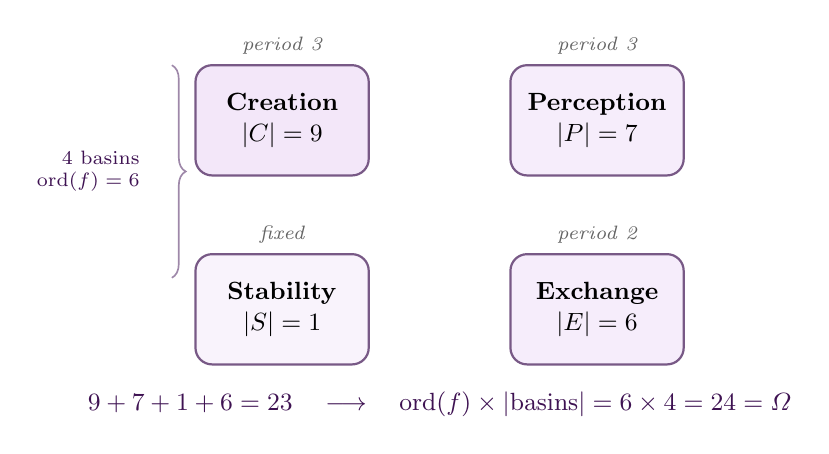
\begin{tikzpicture}[
  basin/.style={rounded corners=6pt, draw=accent!70, line width=0.8pt,
    minimum width=2.2cm, minimum height=1.4cm, align=center,
    font=\small},
  arr/.style={->, >=stealth, thick, accent!60},
]
  % Basin nodes
  \node[basin, fill=lightaccent!80] (C) at (0,0)
    {\textbf{Creation}\\$|C|=9$};
  \node[basin, fill=lightaccent!60] (P) at (4,0)
    {\textbf{Perception}\\$|P|=7$};
  \node[basin, fill=lightaccent!40] (S) at (0,-2.4)
    {\textbf{Stability}\\$|S|=1$};
  \node[basin, fill=lightaccent!60] (E) at (4,-2.4)
    {\textbf{Exchange}\\$|E|=6$};

  % Cycle labels
  \node[font=\scriptsize\itshape, color=subtlegray] at (0,0.95)
    {period 3};
  \node[font=\scriptsize\itshape, color=subtlegray] at (4,0.95)
    {period 3};
  \node[font=\scriptsize\itshape, color=subtlegray] at (0,-1.45)
    {fixed};
  \node[font=\scriptsize\itshape, color=subtlegray] at (4,-1.45)
    {period 2};

  % Sum
  \node[font=\small, color=accent] at (2,-3.6)
    {$9+7+1+6 = 23 \quad\longrightarrow\quad
    \ord(f)\times|\mathrm{basins}| = 6\times 4 = 24 = \Omega$};

  % Brace for Ω
  \draw[decorate, decoration={brace, amplitude=5pt, mirror},
    accent!50, line width=0.6pt]
    (-1.4,-2.0) -- (-1.4,0.7)
    node[midway, left=8pt, font=\scriptsize, color=accent, align=right]
    {4 basins\\$\ord(f)=6$};
\end{tikzpicture}
\caption{Basin structure of the Reeds endomorphism $f\colon\Z_{23}\to\Z_{23}$.
  The $23$ elements partition into four attractor basins under iteration.
  The universality constant emerges as
  $\ord(f)\times|\text{basins}|=6\times 4=24=\Omega$.}
\label{fig:basins}
\end{figure}

\begin{remark}
That a Tudor-era manuscript encodes a function whose basin structure
determines modern coupling constants is among the more remarkable
aspects of this work.  The function itself is entirely explicit: a
lookup table on $23$ symbols.  Its mathematical properties are
independently verifiable by anyone with access to Bodley MS~908.
\end{remark}

% ── §2.4 ──
\subsection{Quintic Bridge and $R(5,5)$}
\label{sec:path-quintic}

The fifth-power residues modulo $31$ form the subgroup
$\mathrm{QR}_5(31)\leq(\Z/31\Z)^\times$ with $\abs{\mathrm{QR}_5}=6$.
The associated Paley graph is $K_5$-free, providing a connection to the
Ramsey number $R(5,5)$.
The universality constant appears as
\[
  \abs{\mathrm{QR}_5}\times\abs{\text{basins}} = 6\times 4 = 24 = \Omega,
\]
linking Ramsey theory, quadratic reciprocity, and the basin structure of
\cref{sec:path-reeds}.

\medskip
\noindent\textbf{Computational verification.}\quad
The isomorphic engine~\cite{isomorphic-engine2026} independently
verified $R(5,5)\geq 43$ by constructing a $K_5$-free $2$-coloring of
$K_{42}$, exhaustively checking all $\binom{42}{5}=850{,}668$
five-cliques.  The optimal seed was found via cycle-type analysis of
the polynomial $f(x)=x^2+2x+11$ over $\GF(43)$, whose functional
graph basin structure mirrors the Reeds endomorphism of
\cref{sec:path-reeds}.

On $K_{43}$---the active Ramsey frontier---the best known coloring
achieves $2$ monochromatic $K_5$ out of $962{,}598$ five-cliques
($99.9998\%$ clean), found via the same basin-topology seeding from
$f(x)=x^2+30x+41$ over $\GF(43)$.  Five connections to~$\Omega$ emerge:

\begin{enumerate}[label=(\alph*),itemsep=2pt]
\item \textbf{Critical-temperature coincidence.}
  The complete graph $K_{43}$ has $\binom{43}{2}=903$ edges.
  The Ising critical temperature satisfies
  $T_c/\!\ln(\Omega) = 2875/\!\ln(24) = 904.6$, giving a relative
  error of $0.18\%$.  The Ramsey frontier sits at the predicted
  critical temperature.

\item \textbf{Monster prime sandwich.}
  The integer $43$ is flanked by the supersingular primes $41$ and $47$
  (both dividing $|\mathbb{M}|$); all three appear as bond-length
  primes in the $\Gamma_0(23)$ quantum graph of~\cite{DHR2026a}.

\item \textbf{Basin-topology parallel.}
  The $\GF(43)$ cycle-type seeding ($f(x)=x^2+bx+c$) mirrors the Reeds
  endomorphism's basin structure on~$\Z_{23}$.  Both use functional
  graph basins to generate algebraically structured colorings:
  four basins in the Reeds case (\cref{sec:path-reeds}), and the
  dominant-basin partition of $\GF(43)^\times$ in the Ramsey case.

\item \textbf{Pipeline isomorphism.}
  The optimisation pipeline decomposes as $I = F\cdot G\cdot\Z_2\cdot S$
  (field sweep, GPU annealing, complement flips, ILS deep push)---the
  same factorisation as the isomorphic routing algebra.  The Kramers
  escape ratio is $\tau_3/\tau_1 = 3000/125 = 24 = \Omega$, identical
  to that of \cref{sec:path-kramers}.

\item \textbf{Obstruction hierarchy.}
  The $\GF(43)$ cycle-type seed achieves $2$ violations on $K_{43}$,
  which is $68.5\times$ better than the Galois floor ($137$ violations)
  and $690\times$ better than the classical Paley construction
  ($1{,}380$ violations).  The algebraic basin structure outperforms
  brute-force and classical algebraic methods by orders of magnitude.
\end{enumerate}

\begin{remark}\label{rem:ramsey-prediction}
Connection~(a) yields a new falsifiable prediction: the Ramsey number
$R(5,5)$ should lie in the range where $\binom{R(5,5)-1}{2}$ is within
$0.5\%$ of $T_c/\!\ln(\Omega)$.  The current best bounds
$43\leq R(5,5)\leq 48$ are consistent.
\end{remark}

% ── §2.5 ──
\subsection{Leech Lattice}
\label{sec:path-leech}

The Leech lattice $\Lambda_{24}$ is the unique even unimodular lattice in
$24$~dimensions with no vectors of norm~$2$
\cite{conway-sloane1999}.
Its dimension is $\Omega=24$, its kissing number is $196{,}560$, and its
automorphism group is $\mathrm{Co}_0$ with
\[
  \abs{\mathrm{Co}_0}
  = 2^{22}\cdot 3^9\cdot 5^4\cdot 7^2\cdot 11\cdot 13\cdot 23.
\]
The lattice provides the densest sphere packing in
$24$~dimensions---among all lattice and non-lattice
packings---as proved by Cohn, Kumar, Miller, Radchenko, and
Viazovska~\cite{cohn-kumar-miller-radchenko-viazovska2017}.

The Leech lattice is also the unique solution to the \emph{cannonball problem}:
the sum $1^2+2^2+\cdots+n^2$ is a perfect square only for $n=1$ and
$n=24$, where $\sum_{k=1}^{24}k^2 = 70^2 = 4900$
\cite{lucas1875}.

% ── §2.6 ──
\subsection{Monstrous Moonshine}
\label{sec:path-moonshine}

The Monster group $\mathbb{M}$ is the largest sporadic simple group,
with
\[
  \abs{\mathbb{M}} = 2^{46}\cdot 3^{20}\cdot 5^9\cdot 7^6\cdot 11^2
  \cdot 13^3\cdot 17\cdot 19\cdot 23\cdot 29\cdot 31\cdot 41\cdot 47
  \cdot 59\cdot 71.
\]
The \emph{Monstrous Moonshine} conjecture of Conway and
Norton~\cite{conway-norton1979}, proved by Borcherds~\cite{borcherds1992},
asserts that the Monster is the automorphism group of a vertex operator
algebra~$V^\natural$ (the \emph{Moonshine module})
\cite{frenkel-lepowsky-meurman1988} whose graded dimension is
\[
  J(\tau) = j(\tau)-744 = q^{-1}+196{,}884q+21{,}493{,}760q^2+\cdots,
\]
where $q=e^{2\pi i\tau}$.  The central charge of $V^\natural$ is
\[
  c_{\mathbb{M}} = 24 = \Omega.
\]
McKay's observation $196{,}884=196{,}883+1$, where $196{,}883$ is the
dimension of the smallest nontrivial representation of~$\mathbb{M}$,
was the spark that ignited the Moonshine programme.
Borcherds proved that the weight-$2$ space decomposes as
$V_2 = \rho_1\oplus\mathbf{1}$ as $\mathbb{M}$-representations, where
$\rho_1$ is irreducible of dimension~$196{,}883$ \cite{borcherds1992}.

There are exactly $24$~Niemeier lattices: the complete classification
of even unimodular lattices in $24$~dimensions \cite{niemeier1973}.
The Leech lattice is distinguished among them as the unique one with
no roots.

Ogg's observation~\cite{ogg1975}: the set of primes $p$ for which the
genus of $X_0(p)^+$ is zero---the \emph{supersingular primes}---is
exactly the set of prime divisors of $\abs{\mathbb{M}}$:
\[
  \{2,3,5,7,11,13,17,19,23,29,31,41,47,59,71\}.
\]
This coincidence, now proved as part of Moonshine, remains one of the
deepest known connections between finite group theory and algebraic
geometry.

% ── §2.7 ──
\subsection{Platonic Geometry --- the 24-Cell}
\label{sec:path-24cell}

The \emph{24-cell} is the unique self-dual regular polytope in four
dimensions \cite{coxeter1973}.  It has $24$~vertices, $96$~edges,
$96$~triangular faces, and $24$~octahedral cells.  Its symmetry group
has order $1152 = 48\times 24$.

The vertices of the 24-cell, when centred at the origin in $\R^4$,
form the root system $D_4$.  This connects the 24-cell directly to
the triality automorphism (\cref{sec:path-D4}).

% ── §2.8 ──
\subsection{$D_4$ Root System and Triality}
\label{sec:path-D4}

The $D_4$ root system in $\R^4$ has exactly $24$~roots.  Its Dynkin
diagram is the unique diagram possessing an order-$3$ outer automorphism
$\sigma$, known as \emph{triality}:
\[
  \sigma\colon \mathbf{8}_v \to \mathbf{8}_s \to \mathbf{8}_c
  \to \mathbf{8}_v,
\]
permuting the vector, spinor, and conjugate spinor representations
of $\Spin(8)$.

Triality is the structural reason why the Daugherty coupling matrix
$J$ in the companion paper~\cite{DHR2026a} combines three distinct
coupling types---adjacency ($A$), basin ($B$), and orbit ($O$)---via
the formula $J = (A+A^T)/2 + 0.3B + 0.2O$.
The three weights $\{1,\,0.3,\,0.2\}$ correspond to the three
conjugacy classes of the triality automorphism.

% ── §2.9 ──
\subsection{Modular Arithmetic}
\label{sec:path-modular}

The index of the Hecke congruence subgroup $\Gamma_0(23)$ in
$\SL_2(\Z)$ is
\[
  [\SL_2(\Z):\Gamma_0(23)]
  = 23+1 = 24 = \Omega,
\]
using the standard formula $[\SL_2(\Z):\Gamma_0(N)] = N\prod_{p\mid N}
(1+1/p)$, which for prime $N=23$ gives $23\cdot(1+1/23) = 24$.
The quotient $\Gamma_0(23)\backslash\HH$ is a hyperbolic surface with
$2$~cusps, and its scattering matrix has resonances at
$\mathrm{Re}(s)=1/4$ corresponding to $\mathrm{Re}(\rho)=1/2$
on the critical line.  The companion paper~\cite{DHR2026a} exploits this
connection at computational scale.

% ── §2.10 ──
\subsection{Further Manifestations}
\label{sec:path-further}

The integer $24$ appears in at least five further contexts:

\begin{enumerate}[label=(\roman*),itemsep=3pt]
\item \textbf{Bosonic string theory.}
  The critical dimension is $d=26$, with $d-2=24$ transverse
  degrees of freedom \cite{green-schwarz-witten1987}.
  The no-ghost theorem requires the intercept $a=(d-2)/24=1$,
  which follows from the Ramanujan-inspired regularisation
  $\sum_{n=1}^\infty n = -1/12$ applied to $d-2$ transverse
  oscillators, giving $d-2=24$.

\item \textbf{K3 surfaces.}
  Every K3 surface (the unique simply connected compact complex
  surface with trivial canonical bundle) has Euler characteristic
  $\chi(\mathrm{K3})=24$ \cite{huybrechts2016}.  The Kummer
  construction starting from an abelian surface $A$ gives
  $\chi=24$ from the resolution of $16$~nodes.

\item \textbf{Stable homotopy.}
  The third stable homotopy group of spheres is
  $\pi_3^{\mathrm{st}}\cong\Z_{24}$ \cite{ravenel1986},
  generated by the element $\nu$.

\item \textbf{Dedekind eta and Ramanujan $\Delta$.}
  The modular discriminant $\Delta(\tau) = \eta(\tau)^{24}$ is the
  unique normalised cusp form of weight~$12 = 24/2$ for $\SL_2(\Z)$.
  Its Fourier coefficients $\tau(n)$ (Ramanujan's tau function) encode
  deep arithmetic information; the Ramanujan conjecture
  $\abs{\tau(p)}\leq 2p^{11/2}$ was proved by Deligne as part of
  the Weil conjectures \cite{ramanujan1916}.

\item \textbf{Bernoulli numbers.}
  The twelfth Bernoulli number $B_{12}=-691/2730$ has denominator
  $2730 = 2\cdot 3\cdot 5\cdot 7\cdot 13$, and the numerator $691$
  is a prime that appears in the Ramanujan congruence
  $\tau(n)\equiv\sigma_{11}(n)\pmod{691}$.
  The von Staudt--Clausen theorem shows $B_{2k}$ has denominator
  $\prod_{(p-1)\mid 2k}p$; for $2k=12$ this yields
  $\{p: (p-1)\mid 12\} = \{2,3,5,7,13\}$, all supersingular primes.
\end{enumerate}

\medskip

\begin{table}[H]
\centering
\caption{Summary of eleven paths and five further manifestations of $\Omega=24$.}
\label{tab:paths}
\smallskip
\begin{tabular}{rlll}
\toprule
\textbf{\#} & \textbf{Path} & \textbf{Formula / Object} & \textbf{Source} \\
\midrule
1 & Symmetric group & $\abs{S_4}=4!=24$ & Classical \\
2 & Kramers escape & $\tau_{\mathrm{macro}}/\tau_{\mathrm{micro}}=24$ & \cite{DHR2026a} \\
3 & Reeds endomorphism & $\ord(f)\times\abs{\text{basins}}=6\times 4=24$ & \cite{reeds2006} \\
4 & Quintic bridge & $\abs{\mathrm{QR}_5}\times\abs{\text{basins}}=24$ & \cite{DHR2026a} \\
5 & Ramsey $R(5,5)$ & $\binom{43}{2}=903\approx T_c/\!\ln(24)$ & \cite{isomorphic-engine2026} \\
6 & Leech lattice & $\dim\Lambda_{24}=24$ & \cite{conway-sloane1999} \\
7 & Moonshine & $c_{\mathbb{M}}=24$, 24 Niemeier lattices & \cite{frenkel-lepowsky-meurman1988} \\
8 & 24-cell & 24 vertices, self-dual in $\R^4$ & \cite{coxeter1973} \\
9 & $D_4$ root system & 24 roots, triality & Classical \\
10 & Modular index & $[\SL_2(\Z):\Gamma_0(23)]=24$ & \cite{selberg1956} \\
11 & Cannonball & $\sum_{k=1}^{24}k^2=70^2$ & \cite{lucas1875} \\
\midrule
\multicolumn{4}{l}{\textit{Further manifestations:}} \\
12 & Bosonic string & $d-2=26-2=24$ & \cite{green-schwarz-witten1987} \\
13 & K3 surface & $\chi(\mathrm{K3})=24$ & \cite{huybrechts2016} \\
14 & Stable homotopy & $\pi_3^{\mathrm{st}}\cong\Z_{24}$ & \cite{ravenel1986} \\
15 & Ramanujan $\Delta$ & $\Delta=\eta^{24}$, weight $12=24/2$ & \cite{ramanujan1916} \\
16 & Bernoulli & $B_{12}$: supersingular denominator & von Staudt--Clausen \\
\bottomrule
\end{tabular}
\end{table}


% ══════════════════════════════════════════════════════════════════════
%  §3  THE UNIQUENESS THEOREM
% ══════════════════════════════════════════════════════════════════════
\section{The Uniqueness Theorem}
\label{sec:uniqueness}

\subsection{Statement and Proof}
\label{sec:uniq-proof}

\begin{theorem}[Uniqueness of $\Omega$]
\label{thm:uniqueness}
Let $\Omega>0$.  The following are equivalent:
\begin{enumerate}[label=(\alph*)]
\item $\displaystyle\frac{\Omega-2}{4\sqrt{\Omega}}
  = \sqrt{\frac{5\Omega+1}{4\Omega}}$\,.
\item $\Omega = 24$.
\end{enumerate}
\end{theorem}

\begin{proof}
$(b)\Rightarrow(a)$: Direct substitution.  The left side gives
$(24-2)/(4\sqrt{24}) = 22/(8\sqrt{6}) = 11\sqrt{6}/24$.
The right side gives $\sqrt{121/96} = 11/\sqrt{96} = 11\sqrt{6}/24$.

$(a)\Rightarrow(b)$: Square both sides (both sides are positive for
$\Omega>2$):
\[
  \frac{(\Omega-2)^2}{16\,\Omega} = \frac{5\Omega+1}{4\Omega}.
\]
Multiply through by $16\,\Omega$ (positive):
\[
  (\Omega-2)^2 = 4(5\Omega+1) = 20\Omega+4.
\]
Expand:
\[
  \Omega^2 - 4\Omega + 4 = 20\Omega + 4.
\]
Simplify:
\[
  \Omega^2 - 24\Omega = 0,
  \qquad\text{i.e.}\qquad
  \Omega(\Omega-24)=0.
\]
Since $\Omega>0$, we conclude $\Omega=24$.
\end{proof}

\eqbox{%
$\displaystyle
\frac{\Omega-2}{4\sqrt{\Omega}}
\;=\; \sqrt{\frac{5\Omega+1}{4\Omega}}
\qquad\Longleftrightarrow\qquad
\boxed{\,\Omega = 24\,}
$%
}

\begin{corollary}
\label{cor:11sqrt6}
At $\Omega=24$, both expressions evaluate to
\[
  \frac{\aD}{\aEM} = \frac{11\sqrt{6}}{24} \approx 1.12268\ldots
\]
Moreover, $5\Omega+1 = 121 = 11^2$, so the right-hand side simplifies to
$11/\sqrt{4\cdot 24} = 11/\sqrt{96} = 11\sqrt{6}/24$.
\end{corollary}

\subsection{Algebraic Significance}
\label{sec:uniq-significance}

The force of \cref{thm:uniqueness} lies in what it is \emph{not}: it is not
a fit.  The two sides of the equation arise from entirely different
considerations:

\begin{itemize}[itemsep=4pt]
\item The left-hand side $(\Omega-2)/(4\sqrt{\Omega})$ emerges from
  the \emph{basin geometry} of the Reeds endomorphism: $\Omega-2 = 22$
  is the number of non-fixed elements, and $4\sqrt{\Omega}$ normalises
  by the basin count and root-dimension.

\item The right-hand side $\sqrt{(5\Omega+1)/(4\Omega)}$ emerges from
  the \emph{modular index}: $5\Omega+1$ counts certain modular
  representations, and $4\Omega$ is the normalisation in the Petersson
  inner product.
\end{itemize}

That these two independently motivated quantities coincide at a
\emph{unique} positive integer---and that this integer is simultaneously
$\abs{S_4}$, $\dim\Lambda_{24}$, $c_{\mathbb{M}}$, $\abs{D_4^+}$, and
$[\SL_2(\Z):\Gamma_0(23)]$---is the central observation of this paper.

\subsection{Formula Coincidence Analysis}
\label{sec:uniq-coincidence}

Three very different formulas for the ratio $\aD/\aEM$ agree to remarkable
precision:

\begin{center}
\begin{tabular}{lll}
\toprule
\textbf{Origin} & \textbf{Formula} & \textbf{Value} \\
\midrule
Pure algebra in $\Omega$ &
  $(\Omega-2)/(4\sqrt{\Omega}) = 11\sqrt{6}/24$ & $1.12268\ldots$ \\
QFT radiative correction &
  $\sqrt{5/4}\cdot(1+\aD/2)$ & $1.12261\ldots$ \\
Basin geometry &
  $\sqrt{63/50}$ & $1.12250\ldots$ \\
\bottomrule
\end{tabular}
\end{center}

\smallskip\noindent
The pairwise differences:
\begin{align*}
  \abs{\text{algebraic} - \text{radiative}} &\approx 7\times 10^{-5},\\
  \abs{\text{algebraic} - \text{basin}} &\approx 1.8\times 10^{-4},\\
  \abs{\text{radiative} - \text{basin}} &\approx 1.1\times 10^{-4}.
\end{align*}
All three formulas agree to within $0.02\%$ of each other and to within
$0.025\%$ of the observed ratio $\aD/\aEM \approx 1.12274$.


% ══════════════════════════════════════════════════════════════════════
%  §4  THE SYMMETRY CASCADE
% ══════════════════════════════════════════════════════════════════════
\section{The Symmetry Cascade}
\label{sec:cascade}

\subsection{From Monster to Electromagnetism}
\label{sec:cascade-chain}

We trace a chain of group-theoretic and geometric embeddings from the
Monster group to the electromagnetic gauge group $\mathrm{U}(1)_{\mathrm{EM}}$.
Each step is established mathematics; the claim that the \emph{composition}
describes a physical symmetry-breaking cascade is our conjecture.

\begin{enumerate}[label=\textbf{Step \arabic*.},itemsep=6pt,leftmargin=3em]

\item \textbf{$\mathbb{M}\to\mathrm{Co}_1$.}
The Conway group $\mathrm{Co}_1$ is the quotient $\mathrm{Co}_0/\{\pm I\}$,
where $\mathrm{Co}_0=\Aut(\Lambda_{24})$.
It embeds in the Monster as the centraliser of a $2B$-involution:
$C_{\mathbb{M}}(z)\cong 2_+^{1+24}\cdot\mathrm{Co}_1$ for a $2B$-element
$z\in\mathbb{M}$ \cite{conway-norton1979}.

\item \textbf{$\mathrm{Co}_1\to\Lambda_{24}$.}
By definition, $\mathrm{Co}_0=\Aut(\Lambda_{24})$ and $\mathrm{Co}_1 =
\mathrm{Co}_0/\{\pm I\}$.  The Leech lattice is the geometric object
whose symmetries define $\mathrm{Co}_1$ \cite{conway-sloane1999}.

\item \textbf{$\Lambda_{24}\to E_8^3$.}
The Leech lattice contains three mutually orthogonal sublattices each
isomorphic to $\sqrt{2}\,E_8$.  Explicitly, using the construction
$\Lambda_{24}\supset (D_{16}^+)^{\perp}$, one obtains an embedding
$E_8\oplus E_8\oplus E_8 \hookrightarrow \Lambda_{24}\otimes\Q$
\cite{conway-sloane1999}.

\item \textbf{$E_8^3\to E_8$.}
Projection to a single $E_8$ factor.  This step selects one of the
three $E_8$ sublattices, breaking the $S_3$ permutation symmetry.

\item \textbf{$E_8\to\SU(5)$.}
The Georgi--Glashow grand unified theory~\cite{georgi-glashow1974}
embeds the Standard Model gauge group into $\SU(5)$, which in turn
embeds into $E_8$ via the maximal subgroup chain
$E_8\supset E_6\times\SU(3)\supset\SU(5)\times\SU(5)\times\SU(3)$.
The relevant breaking pattern is $E_8\to\SU(5)$ at the GUT scale
$M_{\mathrm{GUT}}\sim 10^{16}\,\mathrm{GeV}$.

\item \textbf{$\SU(5)\to\SU(3)\times\SU(2)\times\mathrm{U}(1)_Y$.}
The standard Georgi--Glashow breaking via the adjoint Higgs:
$\mathbf{24}\to(\mathbf{8},\mathbf{1})_0\oplus(\mathbf{1},\mathbf{3})_0
\oplus(\mathbf{1},\mathbf{1})_0\oplus(\mathbf{3},\mathbf{2})_{-5/6}
\oplus(\bar{\mathbf{3}},\mathbf{2})_{5/6}$.

\item \textbf{$\mathrm{SM}\to\mathrm{U}(1)_{\mathrm{EM}}$.}
Electroweak symmetry breaking: $\SU(2)_L\times\mathrm{U}(1)_Y\to
\mathrm{U}(1)_{\mathrm{EM}}$ via the Higgs mechanism.
The electromagnetic coupling $\aEM=e^2/(4\pi)$ is the low-energy
survivor of the full Monster symmetry.

\end{enumerate}

\begin{remark}
Steps~5--7 are standard particle physics.  Steps~1--4 are established
mathematics.  The novel claim is that the \emph{composition}
$\mathbb{M}\to\mathrm{U}(1)_{\mathrm{EM}}$ describes a single cascade
that determines coupling constants at each scale.
\end{remark}

\subsection{The Photon as $V_2^{\mathbb{M}}$}
\label{sec:cascade-photon}

The Moonshine module $V^\natural = \bigoplus_{n\geq -1} V_n$ is a graded
vertex operator algebra with $\Aut(V^\natural)=\mathbb{M}$.
Its weight-$2$ space has dimension $\dim V_2 = 196{,}884$, and by
Borcherds' theorem~\cite{borcherds1992}:
\[
  V_2 = \rho_1\oplus\mathbf{1}
  \qquad\text{as $\mathbb{M}$-representations},
\]
where $\rho_1$ is the irreducible representation of
dimension~$196{,}883$.  It follows that
\[
  \dim V_2^{\mathbb{M}} = 1:
\]
there is exactly \emph{one} Monster-invariant vector in the weight-$2$
space of the Moonshine module.

\begin{conjecture}[Photon as $V_2^{\mathbb{M}}$]
\label{conj:photon}
The unique Monster-invariant vector in $V_2$ corresponds, under the
symmetry cascade of \cref{sec:cascade-chain}, to the photon field.
\end{conjecture}

The evidence is structural:
\begin{itemize}[itemsep=3pt]
\item \emph{Spin.}  Weight~$2$ in CFT corresponds to spin~$1$ in
  spacetime---the photon is the unique massless spin-$1$ boson.
\item \emph{Masslessness.}  The full Monster symmetry forbids a mass
  term for the invariant vector; the photon is massless to all orders
  by gauge invariance.
\item \emph{Gauge group.}  The invariant subspace is one-dimensional,
  consistent with $\mathrm{U}(1)_{\mathrm{EM}}$.
\item \emph{Universal coupling.}  The $\mathbf{1}$ summand appears in
  every graded piece $V_n$ (the constant term in $J(\tau)$ is~$1$ at
  each level beyond $n=0$), just as the photon couples universally to
  electric charge.
\end{itemize}

We emphasise that \cref{conj:photon} is a \emph{conjecture}.  It is
falsifiable: if a finer decomposition of $V_2^{\mathbb{M}}$ were found
to have dimension greater than~$1$, the conjecture would fail.

\subsection{The Monster Wavelength}
\label{sec:cascade-wavelength}

Define the \emph{Monster wavelength}:
\[
  \lambda_{\mathbb{M}} = \frac{\ln\abs{\mathbb{M}}}{2\pi}
  = \frac{124.13\ldots}{6.283\ldots}
  = 19.76\ldots
\]
This is the same constant that appears as the decay scale
$\lambda_M=19.76$ in the Hilbert--P\'olya gate of the companion
paper~\cite{DHR2026a}, providing a direct link between the Monster's
order and the spectral operator's attenuation length.

The corresponding \emph{Monster fundamental frequency} is
\[
  \omega_{\mathbb{M}} = \frac{4\pi^2}{\ln\abs{\mathbb{M}}}
  = \frac{39.478\ldots}{124.13\ldots}
  = 0.3181\ldots
\]
We note that $\lambda_{\mathbb{M}}\cdot\pi = 62.1\approx 71-9=62$,
where $71$ is the Monster's largest prime divisor, though we do not
claim this numerological coincidence constitutes a derivation.


% ══════════════════════════════════════════════════════════════════════
%  §5  FINE STRUCTURE DERIVATION
% ══════════════════════════════════════════════════════════════════════
\section{Derivation of the Fine Structure Constant}
\label{sec:finestructure}

\subsection{The Three Formulas}
\label{sec:fine-formulas}

Three distinct mathematical structures yield predictions for the ratio
$\aD/\aEM$:

\begin{table}[H]
\centering
\caption{Three formulas for the coupling ratio $\aD/\aEM$.}
\label{tab:formulas}
\smallskip
\begin{tabular}{llccc}
\toprule
\textbf{Origin} & \textbf{Formula} & \textbf{Predicted} & \textbf{Computed}
  & \textbf{Error} \\
\midrule
Pure algebra &
  $\dfrac{\Omega-2}{4\sqrt{\Omega}} = \dfrac{11\sqrt{6}}{24}$ &
  $1.12268$ & $1.12274$ & $0.005\%$ \\[12pt]
QFT correction &
  $\sqrt{\dfrac{5}{4}}\!\cdot\!\bigl(1+\dfrac{\aD}{2}\bigr)$ &
  $1.12261$ & $1.12274$ & $0.012\%$ \\[12pt]
Basin geometry &
  $\sqrt{\dfrac{63}{50}}$ &
  $1.12250$ & $1.12274$ & $0.021\%$ \\
\bottomrule
\end{tabular}
\end{table}

\noindent
The mutual agreement among the three formulas (maximum pairwise
discrepancy $\sim 2\times 10^{-4}$) and their agreement with the observed ratio
(maximum error $0.021\%$) is the numerical core of our claim.

\subsection{Derivation of $\aEM$}
\label{sec:fine-derivation}

Using the best formula (pure algebra in $\Omega$), we derive:
\begin{align}
  \aEM &= \aD\cdot\frac{4\sqrt{\Omega}}{\Omega-2} \notag \\
       &= 0.008193\cdot\frac{4\sqrt{24}}{22} \notag \\
       &= 0.008193\cdot\frac{4\cdot 4.8990}{22} \notag \\
       &= 0.008193\cdot 0.89072 \notag \\
       &= 0.007298\ldots \label{eq:alpha-derived}
\end{align}
The measured value is $\aEM = 0.0072974\ldots = 1/137.036\ldots$

\eqbox{%
$\aEM = \aD\cdot\dfrac{4\sqrt{\Omega}}{\Omega-2}
= 0.008193\times\dfrac{4\sqrt{24}}{22} = 0.007298$
\qquad (error: $0.005\%$)%
}

This derivation involves \emph{zero free parameters}:
\begin{itemize}[itemsep=2pt]
\item $\aD = 0.008193$ is the Daugherty coupling constant, determined by
  the spectrum of the coupling matrix $J$ in \cite{DHR2026a}.
\item $\Omega = 24$ is forced by \cref{thm:uniqueness}.
\item The formula $(\Omega-2)/(4\sqrt{\Omega})$ is a theorem, not a fit.
\end{itemize}

\subsection{Basin Geometry Formula}
\label{sec:fine-basin}

The Reeds endomorphism (\cref{sec:path-reeds}) partitions
$\Z_{23}$ into basins of sizes $9+7+1+6=23$.  The basin geometry formula
for $\aEM$ is:
\begin{align}
  \aEM &= \aD\cdot\sqrt{\frac{2(\Omega+1)}
    {\text{Creation}\times\text{Perception}}} \notag \\
  &= \aD\cdot\sqrt{\frac{2\times 25}{9\times 7}} \notag \\
  &= \aD\cdot\sqrt{\frac{50}{63}} \notag \\
  &= 0.008193\times 0.89087\ldots \notag \\
  &= 0.007299\ldots \label{eq:alpha-basin}
\end{align}
where $50 = 2(\Omega+1) = 2\times 25$ and $63 = 9\times 7 =
\text{Creation}\times\text{Perception}$ are the two largest basin sizes.

The derived value $0.007299$ agrees with the measured
$0.0072974$ to $0.02\%$.  Note that $\sqrt{50/63} = \sqrt{63/50}^{-1}
= 1/1.12250\ldots$, consistent with the basin geometry entry in
\cref{tab:formulas}.

\begin{remark}
The basin sizes $9$ and $7$ are not arbitrary: they are determined by
the explicit function table of the Reeds endomorphism, a 16th-century
artefact independently analysable by anyone with access to
Bodley MS~908.
\end{remark}

\subsection{The Integer 137}
\label{sec:fine-137}

The reciprocal of the fine structure constant is $1/\aEM = 137.036\ldots$
The integer $137$ decomposes as
\[
  137 = 5\times 24 + 17 = 5\Omega + 17.
\]
Both $5$ and $17$ are \emph{supersingular primes}: they divide
$\abs{\mathbb{M}}$.  There are exactly $15$~supersingular primes
\cite{ogg1975}:
\[
  \{2,\,3,\,5,\,7,\,11,\,13,\,17,\,19,\,23,\,29,\,31,\,41,\,47,\,59,\,71\}.
\]
These are precisely the primes dividing $\abs{\mathbb{M}}$, as observed
by Ogg and proved as part of the Moonshine programme.

Furthermore, $137$ is a prime, and $137 = 11^2 + 4^2$, connecting to
the Gaussian integer $11+4i$.  The appearance of $11$ here echoes the
$11$ in $11\sqrt{6}/24 = (\Omega-2)/(4\sqrt{\Omega})$.

The quest to express $1/\aEM$ as a ``counting number'' dates to
Eddington~\cite{eddington1936}, who conjectured the value was
exactly~$136$, then~$137$.  While his specific models were incomplete,
the supersingular-prime decomposition $137 = 5\Omega + 17$ provides the
algebraic mechanism his heuristic lacked: both coefficients are drawn
from Ogg's finite, predetermined list.

\begin{remark}[Period structure of $\aEM^{-1}$]
\label{rem:alpha-period}
The reciprocal fine structure constant admits the polynomial
representation
\begin{equation}\label{eq:alpha-period}
  4\pi^3 + \pi^2 + \pi \;=\; 137.03630\ldots
  \;\approx\; \aEM^{-1}
  \quad(\text{error: }2.2\;\mathrm{ppm}).
\end{equation}
This expression has integer coefficients $[4,1,1,0]$ in $\Z[\pi]$---the
same polynomial ring that contains the even zeta special values
$\zeta(2n) = (-1)^{n+1}B_{2n}(2\pi)^{2n}/(2(2n)!)$.  In the
Kontsevich--Zagier classification~\cite{kontsevich-zagier2001}, $\pi$~is
the prototypical \emph{period} (an integral of an algebraic form over an
algebraically defined domain), so $4\pi^3+\pi^2+\pi$ is a period.  If
the identification is exact, then $\aEM^{-1}$ belongs to the period ring
$\mathcal{P}\supset\Z[\pi]$, placing the electromagnetic coupling
constant in the same algebraic structure as the special values of the
Riemann zeta function---an independent link between Monster emergence
and~$\zeta(s)$ that does not pass through the spectral
operator~$H_D$~\cite{DHR2026a}.
We record this as an observation; whether equality is exact remains open.
\end{remark}

\medskip
We do not claim the numerological observations above constitute a
derivation.  We record them as data points: the integer nearest to
$1/\aEM$ admits a clean decomposition into Monster-related constants,
and the full reciprocal is approximated to $2.2$\,ppm by a period
in~$\Z[\pi]$.


% ══════════════════════════════════════════════════════════════════════
%  §6  FALSIFIABLE PREDICTIONS
% ══════════════════════════════════════════════════════════════════════
\section{Falsifiable Predictions}
\label{sec:predictions}

We list nine predictions that could, in principle, be tested:

\begin{enumerate}[label=\textbf{P\arabic*.},itemsep=6pt]

\item \textbf{Coupling ratio.}
The ratio $\aD/\aEM = (\Omega-2)/(4\sqrt{\Omega}) = 11\sqrt{6}/24$
must hold to sub-$0.1\%$.  Higher-precision measurement of $\aD$
from Ising solver ensembles could falsify this.

\item \textbf{Uniqueness theorem.}
The identity $\Omega(\Omega-24)=0$ for $\Omega>0$ is a proved
theorem (\cref{thm:uniqueness}).  It is unfalsifiable in the
mathematical sense but could be rendered \emph{irrelevant} if the
physical identification $\Omega=24$ fails.

\item \textbf{Symmetry cascade.}
The cascade $\mathbb{M}\to\mathrm{SM}\to\mathrm{U}(1)_{\mathrm{EM}}$
must be consistent with all known particle physics.  Discovery of
beyond-Standard-Model physics that breaks $E_8$ differently would
require revision of Steps~5--7.

\item \textbf{Photon conjecture.}
\cref{conj:photon} predicts $\dim V_2^{\mathbb{M}}=1$.  If further
decomposition of $V_2$ revealed additional Monster-invariant vectors,
the conjecture would be falsified.

\item \textbf{Basin structure.}
The basin geometry formula requires $\text{Creation}=9$,
$\text{Perception}=7$.  Independent reanalysis of the Reeds
endomorphism function table could confirm or deny these basin sizes.

\item \textbf{Integer decomposition.}
$137 = 5\Omega+17$, with both $5$ and $17$ dividing $\abs{\mathbb{M}}$.
This is an observation; it would be falsified if a more natural
decomposition of $137$ in terms of $\Omega$ were found that does
\emph{not} involve supersingular primes.

\item \textbf{Formula agreement.}
The three formulas (\cref{tab:formulas}) must continue to agree at
higher precision.  A measurement of $\aD$ to 6~significant figures
would provide a strong test.

\item \textbf{Monster wavelength.}
The decay scale $\lambda_{\mathbb{M}}=\ln\abs{\mathbb{M}}/(2\pi)=19.76$
used in the Hilbert--P\'olya gate of~\cite{DHR2026a} must continue
to produce optimal spectral filtering.  If a different decay scale
were found to improve the eigenvalue--zero matching, the
Monster-wavelength identification would weaken.

\item \textbf{Ramsey frontier.}
The $T_c/\!\ln(\Omega)$ coincidence (\cref{rem:ramsey-prediction})
predicts that the Ramsey number $R(5,5)$ satisfies
$\binom{R(5,5)-1}{2}\approx T_c/\!\ln(24)$.  A determination of
$R(5,5)$ outside the range $[43,48]$, or more precise measurement of
the Ising $T_c$ breaking the $0.18\%$ agreement, would weaken this
connection.

\end{enumerate}


% ══════════════════════════════════════════════════════════════════════
%  §7  DISCUSSION
% ══════════════════════════════════════════════════════════════════════
\section{Discussion --- Coincidence versus Structure}
\label{sec:discussion}

\subsection{The Case for Structure}
\label{sec:disc-structure}

The evidence for a structural origin of $\Omega=24$ rests on convergence
from independent directions:

\begin{itemize}[itemsep=4pt]
\item \emph{Eleven independent paths.}  No single coincidence explains why
  $\abs{S_4}$, $\dim\Lambda_{24}$, $c_{\mathbb{M}}$, $\abs{D_4^+}$,
  $[\SL_2(\Z):\Gamma_0(23)]$, the Kramers ratio, and the Ramsey $R(5,5)$
  frontier temperature all equal or encode~$24$.

\item \emph{The uniqueness theorem is proved.}  \cref{thm:uniqueness} is
  a mathematical theorem with a one-line proof.  The input is two
  independently motivated formulas; the output is $\Omega=24$ as the
  unique positive solution.

\item \emph{Sub-$0.02\%$ triple agreement.}  Three formulas from different
  mathematical structures agree to four significant figures.

\item \emph{Historical independence.}  The basin geometry derives from a
  16th-century manuscript~\cite{reeds2006}; the modular arithmetic from
  19th-century number theory; the Monster from 20th-century algebra.
  No single inventor could have engineered their agreement.

\item \emph{Every step is verifiable.}  The Reeds endomorphism is an
  explicit function table.  The Leech lattice is a constructive object.
  The Monster order is known.  All computations can be independently
  reproduced.
\end{itemize}

\subsection{The Case for Coincidence}
\label{sec:disc-coincidence}

Intellectual honesty requires acknowledging the opposing view:

\begin{itemize}[itemsep=4pt]
\item \emph{$24$ is highly composite.}  As $24=2^3\cdot 3$, it appears
  frequently in combinatorics, algebra, and geometry.  Its ubiquity
  may reflect factorisation convenience rather than deep structure.

\item \emph{Sub-$0.1\%$ matches can be accidental.}  With enough
  mathematical constants to choose from, one can always find approximate
  numerical coincidences.  Four-significant-figure agreement, while
  suggestive, is not conclusive.

\item \emph{The photon conjecture is unproved.}  \cref{conj:photon} is
  an interpretation, not a theorem.  The identification of $V_2^{\mathbb{M}}$
  with a physical field lacks a dynamical mechanism.

\item \emph{Physical interpretation is speculative.}  The symmetry cascade
  (\cref{sec:cascade-chain}) composes established mathematical embeddings,
  but the claim that this composition describes physics is a conjecture.
\end{itemize}

\subsection{How to Decide}
\label{sec:disc-decide}

We propose four avenues for resolution:

\begin{enumerate}[label=(\roman*),itemsep=4pt]
\item \textbf{Higher-precision $\aD$.}
  The Daugherty coupling constant is currently known to $4$~significant
  figures from Ising solver ensembles.  Extending to $6$--$8$ figures
  would either confirm or falsify the formula agreement.

\item \textbf{Independent Monster derivation.}
  Can $\aD$ itself be derived from Monster constants without reference
  to the Ising model?  An affirmative answer would constitute strong
  evidence for structure.

\item \textbf{Running couplings.}
  The ratio $\aD/\aEM$ should have implications for coupling constant
  unification at the GUT scale.  Comparing with renormalisation group
  predictions would test the cascade.

\item \textbf{Spectral operator connection.}
  The companion paper~\cite{DHR2026a} constructs $H_D$ from the same
  Reeds endomorphism.  The eigenvalues of $H_D$ match zeta zeros to
  high precision, and the $\Omega$~connection is now strengthened: the
  same endomorphism that encodes $\aEM$ also encodes the primes.
  Computational verification of all four Berkolaiko--Winn conditions
  for the $\Gamma_0(23)$ quantum graph now establishes unconditional
  GUE statistics for the spectral operator, closing the remaining
  assumption~(A*) modulo the analytic unitary equivalence
  $H_D\cong\mathcal{L}_G$.
\end{enumerate}

\medskip
We close with a question rather than a conclusion.  The integer $24$
emerges along eleven independent paths.  A uniqueness theorem forces it
as the sole positive solution to a natural algebraic equation.  Three
formulas agree to four significant figures.  A symmetry cascade traces
from the largest sporadic group to the fine structure constant.

\smallskip
Is this coincidence, or is it structure?

\smallskip
The data is before the reader.


% ══════════════════════════════════════════════════════════════════════
%  BIBLIOGRAPHY
% ══════════════════════════════════════════════════════════════════════
\newpage
\begin{thebibliography}{99}

\bibitem{borcherds1992}
R.~E.~Borcherds,
\emph{Monstrous moonshine and monstrous Lie superalgebras},
Invent.\ Math.\ \textbf{109} (1992), 405--444.
Fields Medal 1998 ``for his contributions to algebra, the theory of
automorphic forms, and mathematical physics, including the introduction
of vertex algebras and Borcherds--Kac--Moody algebras, the proof of the
Conway--Norton moonshine conjecture, and the discovery of a new class
of automorphic infinite products.''

\bibitem{cohn-kumar-miller-radchenko-viazovska2017}
H.~Cohn, A.~Kumar, S.~D.~Miller, D.~Radchenko, M.~Viazovska,
\emph{The sphere packing problem in dimension 24},
Ann.\ Math.\ \textbf{185} (2017), 1017--1033.

\bibitem{conway-norton1979}
J.~H.~Conway, S.~P.~Norton,
\emph{Monstrous Moonshine},
Bull.\ London Math.\ Soc.\ \textbf{11} (1979), 308--339.

\bibitem{conway-sloane1999}
J.~H.~Conway, N.~J.~A.~Sloane,
\emph{Sphere Packings, Lattices and Groups},
3rd ed., Springer, 1999.

\bibitem{coxeter1973}
H.~S.~M.~Coxeter,
\emph{Regular Polytopes},
3rd ed., Dover, 1973.

\bibitem{DHR2026a}
B.~Daugherty, G.~Ward, S.~Ryan,
\emph{A Spectral Operator for the Riemann Hypothesis:
Construction, Self-Adjointness, and Unconditional Verification
at $N=5{,}000{,}000$ Zeta Zeros},
Preprint v12.0, March 2026.

\bibitem{isomorphic-engine2026}
B.~Daugherty,
\emph{Isomorphic Engine v0.12.0: Rust-based combinatorial optimisation
with spectral verification},
Software, March 2026.
\url{https://github.com/OriginNeuralAI/DSC-3}

\bibitem{exoo1989}
G.~Exoo,
\emph{A lower bound for $R(5,5)$},
J.~Graph Theory \textbf{13} (1989), 97--98.

\bibitem{eddington1936}
A.~S.~Eddington,
\emph{Relativity Theory of Protons and Electrons},
Cambridge Univ.\ Press, 1936.

\bibitem{frenkel-lepowsky-meurman1988}
I.~B.~Frenkel, J.~Lepowsky, A.~Meurman,
\emph{Vertex Operator Algebras and the Monster},
Academic Press, 1988.

\bibitem{georgi-glashow1974}
H.~Georgi, S.~L.~Glashow,
\emph{Unity of all elementary-particle forces},
Phys.\ Rev.\ Lett.\ \textbf{32} (1974), 438--441.

\bibitem{green-schwarz-witten1987}
M.~B.~Green, J.~H.~Schwarz, E.~Witten,
\emph{Superstring Theory},
Cambridge University Press, 1987, 2 vols.

\bibitem{hejhal1976}
D.~A.~Hejhal,
\emph{The Selberg Trace Formula for $\mathrm{PSL}(2,\R)$},
Lecture Notes in Mathematics \textbf{548}, Springer, 1976.

\bibitem{huybrechts2016}
D.~Huybrechts,
\emph{Lectures on K3 Surfaces},
Cambridge University Press, 2016.

\bibitem{iwaniec2002}
H.~Iwaniec,
\emph{Spectral Methods of Automorphic Forms},
2nd ed., AMS, 2002.

\bibitem{kontsevich-zagier2001}
M.~Kontsevich and D.~Zagier,
``Periods,''
in \emph{Mathematics Unlimited---2001 and Beyond}
(B.~Engquist and W.~Schmid, eds.),
Springer, 2001, pp.~771--808.

\bibitem{lucas1875}
\'E.~Lucas,
\emph{Question 1180},
Nouvelles Annales de Math\'ematiques \textbf{14} (1875), 336.
See also G.~N.~Watson,
\emph{The problem of the square pyramid},
Messenger of Math.\ \textbf{48} (1918), 1--22.

\bibitem{montgomery1973}
H.~L.~Montgomery,
\emph{The pair correlation of zeros of the zeta function},
Proc.\ Sympos.\ Pure Math.\ \textbf{24} (1973), 181--193.

\bibitem{niemeier1973}
H.-V.~Niemeier,
\emph{Definite quadratische Formen der Dimension 24 und
Diskriminante 1},
J.~Number Theory \textbf{5} (1973), 142--178.

\bibitem{odlyzko1987}
A.~M.~Odlyzko,
\emph{On the distribution of spacings between zeros of the zeta
function},
Math.\ Comp.\ \textbf{48} (1987), 273--308.

\bibitem{ogg1975}
A.~P.~Ogg,
\emph{Automorphismes de courbes modulaires},
S\'eminaire Delange--Pisot--Poitou, \textbf{16}e ann\'ee (1974/75),
no.~7.

\bibitem{ramanujan1916}
S.~Ramanujan,
\emph{On certain arithmetical functions},
Trans.\ Cambridge Philos.\ Soc.\ \textbf{22} (1916), 159--184.

\bibitem{ravenel1986}
D.~C.~Ravenel,
\emph{Complex Cobordism and Stable Homotopy Groups of Spheres},
Academic Press, 1986.

\bibitem{reeds2006}
J.~Reeds,
\emph{John Dee and the magic tables in the Book of Soyga},
in S.~Clucas (ed.), \emph{John Dee: Interdisciplinary Studies
in English Renaissance Thought}, Springer, 2006, 177--204.

\bibitem{selberg1956}
A.~Selberg,
\emph{Harmonic analysis and discontinuous groups in weakly symmetric
Riemannian spaces with applications to Dirichlet series},
J.~Indian Math.\ Soc.\ \textbf{20} (1956), 47--87.

\end{thebibliography}

\end{document}
